\documentclass{article}
\usepackage{amsmath}
\usepackage{amssymb}
\usepackage{graphicx}
\usepackage{hyperref}
\usepackage[version=4]{mhchem}


\begin{document}
(2004 AMC 10B Problem 20) In \(\triangle A B C\) points \(D\) and \(E\) lie on \(B C\) and \(A C\), respectively. Suppose that \(A D\) and \(B E\) intersect at T so that \(A T / D T=3\) and \(B T / E T=4\). What is the value of \(C D / B D\) ?\\
(A) \(\frac{1}{8}\)\\
(B) \(\frac{2}{9}\)\\
(C) \(\frac{3}{10}\)\\
(D) \(\frac{4}{11}\)\\
(E) \(\frac{5}{12}\)

Solution: (D).\\
\centering
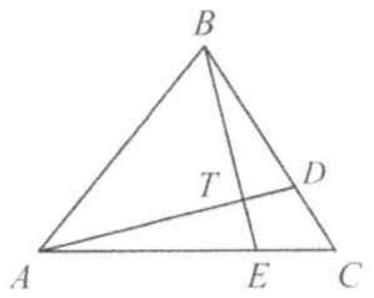
\includegraphics[width=\textwidth]{images/104.jpg}

Method 1:\\
Let \(F\) be a point on \(A C\) such that \(D F\) is parallel to \(B E\). Let \(B T=4 x\) and \(E T=x\).\\
Because \(\triangle A T E\) and \(\triangle A D F\) are similar, we have\\
\(\frac{D F}{x}=\frac{A D}{A T}=\frac{4}{3}\) and \(D F=\frac{4 x}{3}\).\\
Also, \(\triangle B E C\) and \(\triangle D F C\) are similar, so\\
\(\frac{C D}{B C}=\frac{D F}{B E}=\frac{4 x / 3}{5 x}=\frac{4}{15}\).\\
\centering
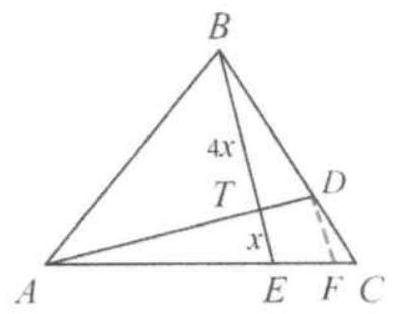
\includegraphics[width=\textwidth]{images/104(1).jpg}

Thus \(\frac{C D}{B C}=\frac{C D / B C}{1-C D / B C}=\frac{4 / 15}{1-4 / 15}=\frac{4}{11}\).\\
Method 2:\\
Let \(F\) be a point on \(B E\) such that \(D F\) is parallel to \(A C\). Let \(B T=4 x\) and \(E T=x\).\\
Let \(A T=3 y\) and \(D T=y\).\\
Because \(\triangle A T E\) and \(\triangle D T F\) are similar, we have\\
\(\frac{A T}{D T}=\frac{E T}{F T}=\frac{3}{1} \Rightarrow \frac{x}{F T}=\frac{3}{1} \Rightarrow F T=\frac{x}{3}\).\\
So \(E F=x+\frac{x}{3}=\frac{4}{3} x\) and \(B F=4 x-\frac{x}{3}=\frac{11}{3} x\)\\
\centering
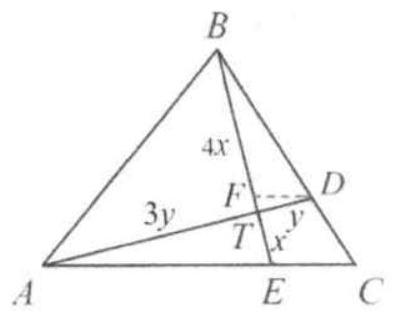
\includegraphics[width=\textwidth]{images/104(2).jpg}

Also, \(\triangle B E C\) and \(\triangle B F D\) are similar, so\\
\(\frac{B F}{E F}=\frac{B D}{C D} \quad \Rightarrow \quad \frac{\frac{11}{3} x}{\frac{4 x}{3}}=\frac{B D}{C D} \quad \Rightarrow \frac{C D}{B C}=\frac{4}{11}\).


(1) \(\div(2): \frac{C D}{B D}=\frac{4}{11}\).

Method 5:\\
Let \(F\) be a point on \(A C\) such that \(T F\) is parallel to \(B C\). Let \(B T=4 x\) and \(E T=x\). Let \(A T=3 y\) and \(D T=y\).

Because \(\triangle A T F\) and \(\triangle A D C\) are similar, we have

\[
\frac{A T}{A D}=\frac{F T}{C D} \Rightarrow \frac{3 y}{4 y}=\frac{F T}{C D} \Rightarrow \frac{F T}{C D}=\frac{3}{4}
\]

Also, \(\triangle B E C\) and \(\triangle T E F\) are similar, so\\
\(\frac{F T}{B C}=\frac{E T}{B E} \quad \Rightarrow \quad \frac{F T}{B D+C D}=\frac{x}{5 x}\)\\
\centering
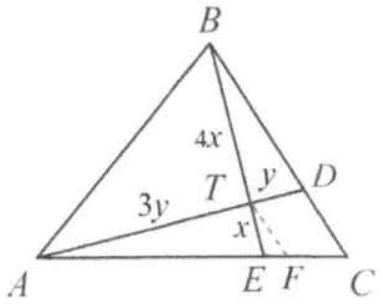
\includegraphics[width=\textwidth]{images/105(1).jpg}

\[
\Rightarrow \quad \frac{F T}{B D+C D}=\frac{1}{5}
\]

(1) \(\div\) (2): \(\frac{B D+C D}{C D}=\frac{15}{4} \quad \Rightarrow \frac{B D}{C D}+1=\frac{15}{4}\)

\[
\Rightarrow \frac{B D}{C D}=\frac{11}{4} \Rightarrow \frac{C D}{B D}=\frac{4}{11} .
\]

Method 6:\\
Let \(F\) be a point on \(B C\) such that \(T F\) is parallel to \(B C\). Let \(B T=4 x\) and \(E T=x\). Let \(A T=3 y\) and \(D T=y\).

Because \(\triangle A D C\) and \(\triangle T D F\) are similar, we have\\
\(\frac{A T}{C F}=\frac{D T}{D F} \Rightarrow \frac{3 y}{C F}=\frac{y}{D F} \Rightarrow \frac{C F}{D F}=3 \Rightarrow\)\\
\(\frac{C D-D F}{D F}=3 \Rightarrow \frac{C D}{D F}=4\)\\
\centering
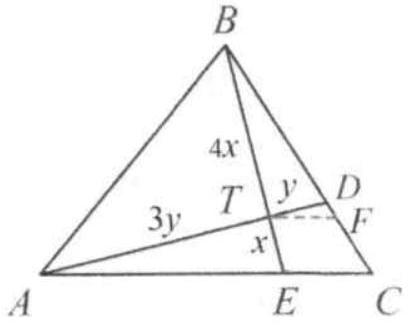
\includegraphics[width=\textwidth]{images/105.jpg}

Because \(\triangle B T F\) and \(\triangle B E C\) are similar, so\\
\(\frac{B T}{T E}=\frac{B F}{C F} \quad \Rightarrow \quad \frac{4 x}{x}=\frac{B F}{C F}=4\)\\
\(\frac{B F}{C F}=\frac{B D+D F}{C F}=4 \Rightarrow \quad \frac{B D+D F}{3 D F}=4 \quad \Rightarrow \quad \frac{B D}{D F}+1=12\)\\
\(\Rightarrow \quad \frac{B D}{D F}=11\)\\
(1) \(\div(2): \frac{C D}{B D}=\frac{4}{11}\).


\end{document}
